\documentclass[12pt,a4paper]{article}

% Encoding and font setup
\usepackage[utf8]{inputenc}
\usepackage[T1]{fontenc}
\usepackage{mathptmx} % Times font with math support
\usepackage{microtype} % Better typography

% Geometry and spacing
\usepackage{geometry}
\geometry{a4paper, margin=0.8in}
\usepackage{setspace}
\onehalfspacing

% Math packages
\usepackage{amsmath, amssymb, amsthm, mathtools, bm}

% Hyperlinks
\usepackage{hyperref}
\hypersetup{
    colorlinks=true,
    linkcolor=blue,
    citecolor=blue,
    urlcolor=blue
}

% Lists and formatting
\usepackage{enumitem} % better lists
\usepackage{tocloft}  % customize ToC

% Figures and diagrams
\usepackage{graphicx}
\usepackage{xcolor}
\usepackage{tikz}
\usetikzlibrary{positioning, shapes, arrows, shadows}

% Theorem environments
\theoremstyle{definition}
\newtheorem{definition}{Definition}[subsection]
\newtheorem{theorem}{Theorem}[subsection]
\newtheorem{lemma}{Lemma}[subsection]
\newtheorem{proposition}{Proposition}[subsection]
\newtheorem{remark}{Remark}[subsection]

% Common math shortcuts (minimal set)
\newcommand{\R}{\mathbb{R}}
\newcommand{\vect}[1]{\bm{#1}}
\newcommand{\norm}[1]{\left\lVert #1 \right\rVert}

% Title page
\begin{document}

\begin{titlepage}
    \centering
    \vspace*{1cm}
    {\huge \textbf{From Projection to Perception: \\ A Mathematical Exploration of \\ Shadow-based Neural Reconstruction}\par}
    \vspace{1.5cm}
    {\normalsize
    A research report submitted to the Scientific Committee of the Hang Lung Mathematics Award\par}
    \vspace{1cm}
    {\normalsize \textbf{Team Number}\par 2596873\par}
    \vspace{0.5cm}
    {\normalsize \textbf{Team Members}\par Wong Yuk To, Hung Kwong Lam \\ Cheung Tsz Lung, Chan Ngo Tin, Zhou Lam Ho\par}
    \vspace{0.5cm}
    {\normalsize \textbf{Teacher}\par Mr. Chan Ping Ho\par}
    \vspace{0.5cm}
    {\normalsize \textbf{School}\par Po Leung Kuk Celine Ho Yam Tong College\par}
    \vspace{0.5cm}
    {\normalsize \textbf{Date}\par \today\par}
    \vfill

    \begin{abstract}
    \noindent
    This paper explores \textsc{ShadowNeuS} \hyperlink{[LWX23]}{[LWX23]}, a neural network that reconstructs 3D geometry from single-view camera images using shadow and light cues. Unlike traditional 3D reconstruction methods relying on multi-view cameras or sensors, \textsc{ShadowNeuS} leverages a neural signed distance field (SDF) for accurate 3D geometry reconstruction. We analyze the training process and uncover its connections to projective geometry, spatial reasoning in $\R^3$, and the neural network's learned geometric representation of space.
    \end{abstract}
\end{titlepage}

\tableofcontents
\newpage

\section{Introduction}
\subsection{Background}
3D reconstruction is the process of recovering the shape and structure of an object in \(\mathbb{R}^3\) from measured data. It has broad applications in medical imaging (MRI, CT), robotics, augmented/virtual reality (AR/VR), and cultural heritage preservation. Most conventional methods rely heavily on geometric and physical modeling techniques and require rich spatial data obtained through multi-view camera setups, LiDAR sensors, or photogrammetry.

\subsection{Motivation}
Traditional approaches typically depend on \textbf{multiple viewpoints or depth sensors}, which is costly and complex. This leads to the question: \textbf{Is it possible to reconstruct 3D geometry from a single fixed camera?} A single image inherently lacks depth information, and multiple 3D points can project to the same 2D pixel location (as discussed in Section \ref{sec: illposed}). Therefore, additional cues are essential to resolve this ambiguity. \\
In exploring this problem, we discovered the paper \textit{ShadowNeuS: Neural SDF Reconstruction by Shadow Ray Supervision} \hyperlink{[LWX23]}{[LWX23]} by Jingwang Ling, Zhibo Wang, and Feng Xu. Their approach demonstrates that leveraging neural signed distance fields and supervising the network with shadow ray information under varying lighting enables accurate 3D reconstruction from single-view images. Motivated by their work, we present a study analyzing their method and propose a 1D-to-2D experimental validation to examine our understanding.

\section{Fundamentals of 3D Reconstruction from 2D Images}
\subsection{3D Reconstruction in Computer Vision}
According to an article on Medium \hyperlink{[VK23]}{[VK23]}, 3D computer vision is a field of computer science focusing on the analysis, interpretation, and understanding of three-dimensional visual data. \\
The article highlights a traditional approach for 3D reconstruction:

\begin{minipage}{0.5\textwidth}
    \textbf{Structure from Motion (SfM)} \\
    Recover the 3D structure by estimating camera \\ positions from multiple images.
\end{minipage}
\hspace{0.5cm}
\begin{minipage}{0.5\textwidth}
    \centering
    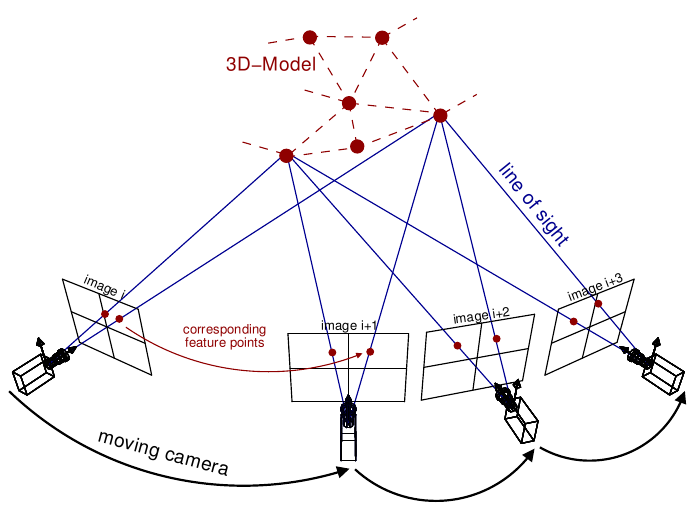
\includegraphics[height=0.2\textheight]{SfM.png} \\
    \hyperlink{[Fig 1]}{\textbf{Figure 1.}} Structure from Motion
\end{minipage}

\newpage

\subsection{Information Encoded in a Single-View Image}
When only single-view is available, the following information remains exploitable:

\begin{itemize}[noitemsep, topsep=0pt, parsep=0pt, partopsep=0pt]
    \item \textbf{Pixel position \((u, v)\)} — relates to a 3D ray from camera to that pixel
    \item \textbf{Color / intensity} — encodes surface information (material, orientation, etc.)
    \item \textbf{Embedded features} (edges, recognized objects) — encode geometry cues
\end{itemize}

\begin{center}
\begin{minipage}{0.35\textwidth}
    \centering
    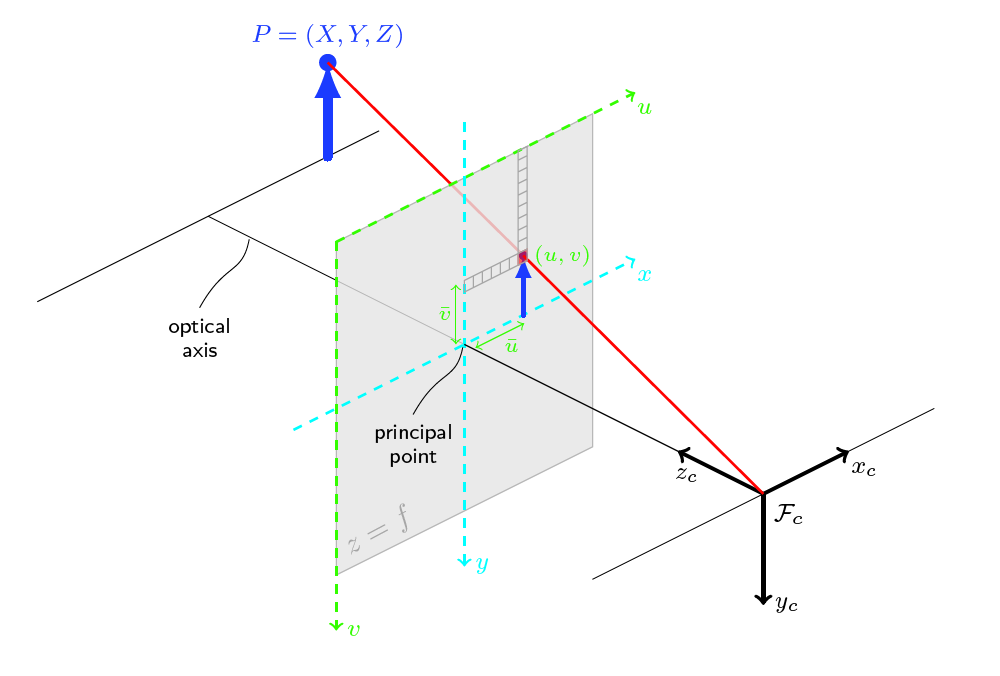
\includegraphics[width=\textwidth]{pixel_position.png} \\
    \hyperlink{[Fig 2]}{\textbf{Figure 2.}} Ray from camera to pixel
\end{minipage}
\hfill
\begin{minipage}{0.2\textwidth}
    \centering
    
\includegraphics[width=\textwidth]{color_intensity.jpg} \\
    \hyperlink{[Fig 3]}{\textbf{Figure 3.}} Texture
\end{minipage}
\hfill
\begin{minipage}{0.35\textwidth}
    \centering
    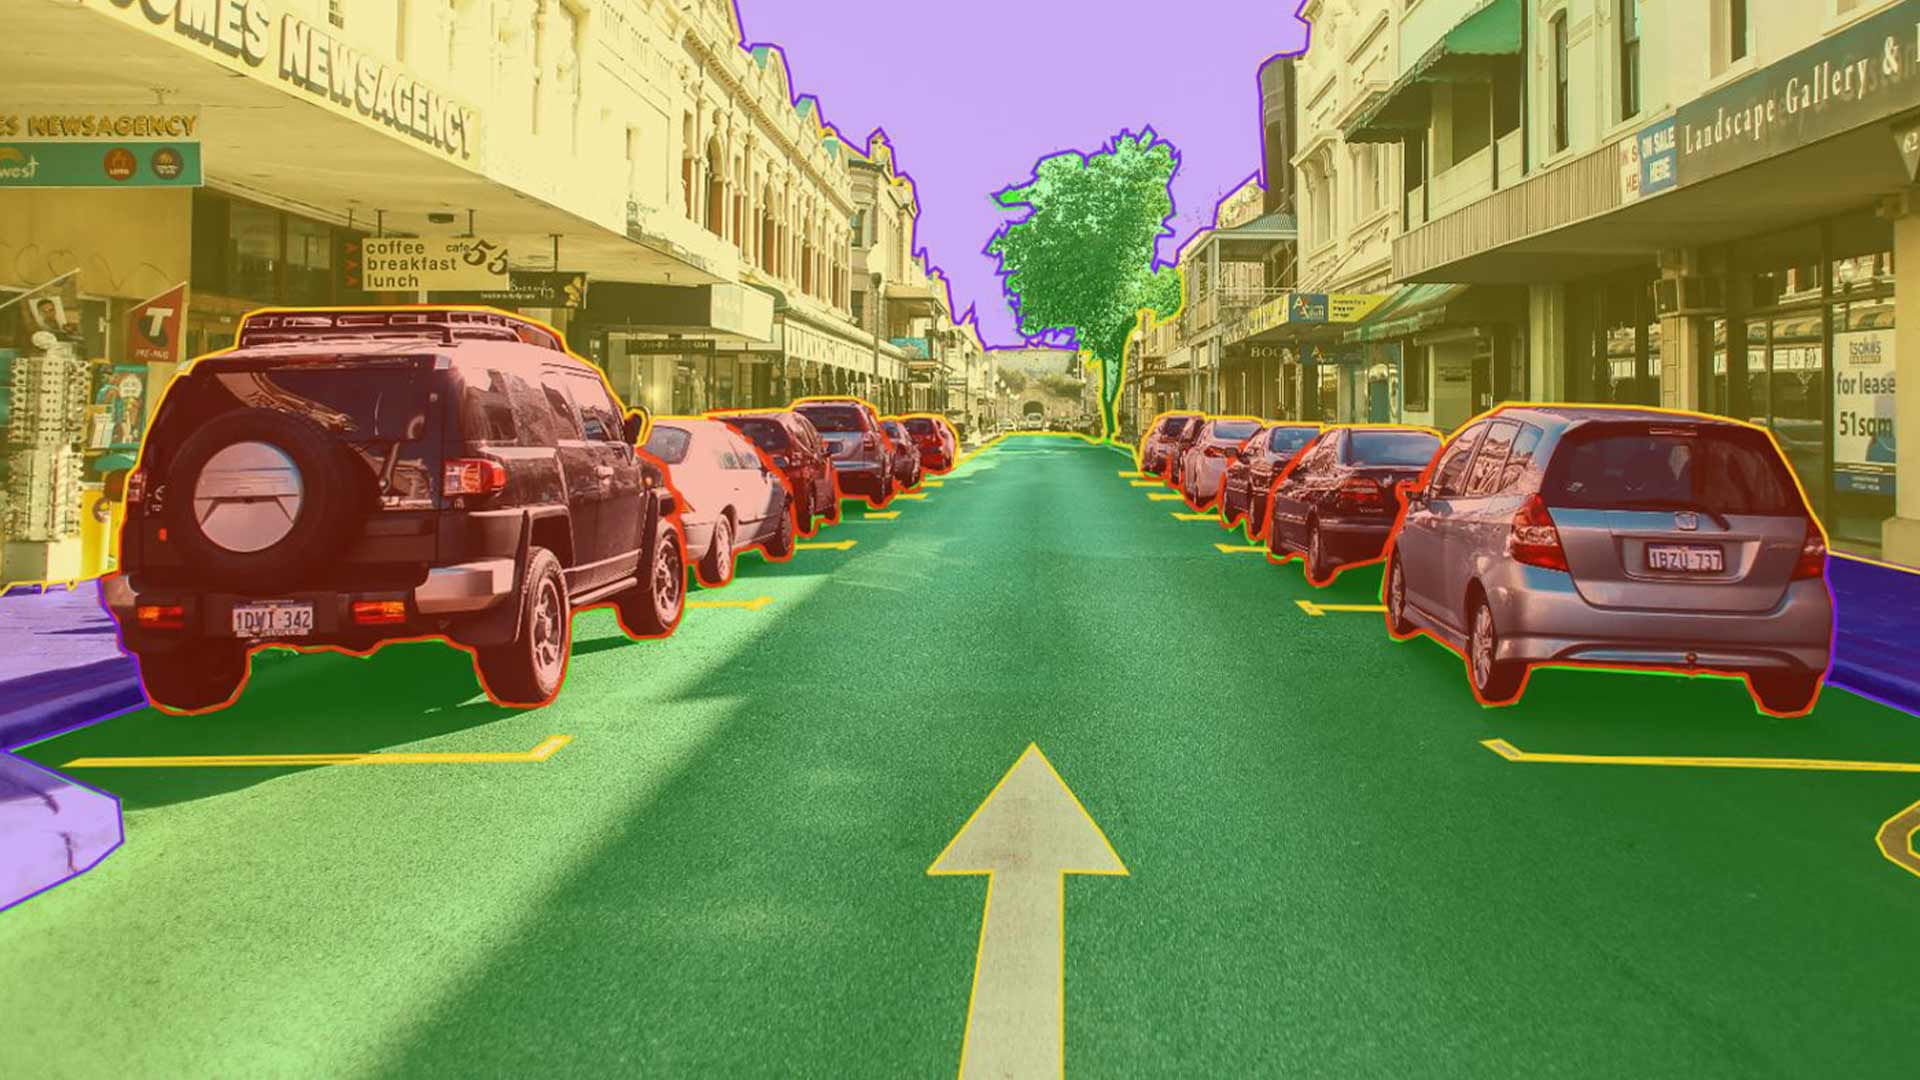
\includegraphics[width=\textwidth]{embedded_features.jpg} \\
    \hyperlink{[Fig 4]}{\textbf{Figure 4.}} Object segmentation (YOLO)
\end{minipage}
\end{center}

\vspace{-1em}

\subsection{Forward Projection: Mapping from 3D to 2D} \label{sec:forward_projection}
\vspace{-0.5em}
In this section, we want to show that mapping from a 3D point \(\vect{P} = (x,y,z)^\mathsf{T} \in \R^3\) in the world coordinate system onto a 2D image pixel coordinate \(\vect{p} = (u,v)^\mathsf{T} \in \R^2\) is a projection-like process.

\noindent\textbf{Extrinsic parameters:} define the camera's position and orientation relative to the world:
\vspace{-0.5em}
\begin{equation}
C = \underbrace{\begin{bmatrix} C_x \\ C_y \\ C_z \end{bmatrix} \in \R^3}_{\substack{\text{Camera center}}}, \quad
R = \underbrace{
\begin{bmatrix}
r_{11} & r_{12} & r_{13} \\
r_{21} & r_{22} & r_{23} \\
r_{31} & r_{32} & r_{33}
\end{bmatrix} \in \mathrm{SO}(3)
}_{\substack{\text{Rotation matrix}}}, \quad
t = \underbrace{-R C \in \R^3}_{\substack{\text{Translation vector}}}
\label{eq:extrinsic}
\end{equation}

\noindent\textbf{Intrinsic parameters:} encode the internal camera geometry:
\vspace{-0.5em}
\begin{equation}
K = \begin{bmatrix}
f_x & 0 & c_x \\
0 & f_y & c_y \\
0 & 0 & 1
\end{bmatrix} \in \R^{3 \times 3}
\label{eq:intrinsic}
\end{equation}
where \((f_x, f_y)\) are the focal lengths in pixels, and \((c_x, c_y)\) is the principal point (image center).

The forward projection consists of three steps:
\begin{enumerate}[noitemsep, topsep=0pt, parsep=0pt, partopsep=0pt]
    \item Transform \(\vect{P}\) from world coordinates to camera coordinates: \(\vect{P}_{\text{cam}} = R (\vect{P} - C) = R \vect{P} + t\).
    \item Project camera coordinates to homogeneous image coordinates: \(\vect{P}_{\text{hom}} = K \vect{P}_{\text{cam}} = \begin{bmatrix} p_x' \\ p_y' \\ z' \end{bmatrix}\).
    \vspace{-0.5em}
    \item Normalize by depth \(z'\) to get pixel coordinates: \(\vect{p} = \frac{1}{z'} \begin{bmatrix} p_x' \\ p_y' \end{bmatrix}, \quad z' \neq 0\).
\end{enumerate}

Combined expressions:
\begin{equation}
\boxed{
\vect{P}_{\text{hom}} = \begin{bmatrix} p_x' \\ p_y' \\ z' \end{bmatrix} = K [R \mid t] \begin{bmatrix} \vect{P} \\ 1 \end{bmatrix}, \quad
\vect{p} = \frac{1}{z'} \begin{bmatrix} p_x' \\ p_y' \end{bmatrix}
}
\label{eq:forward}
\end{equation}

\newpage

\subsection{The Inverse Problem: From 2D Image to 3D World} \label{sec:inverse_problem}

After understanding the forward projection process, 3D reconstruction can be viewed as the inverse calculation: recovering 3D points from their 2D image projections. \\  
We now tackle the challenge of inverting the projection function introduced in Section \ref{sec:forward_projection}.

\begin{lemma}[Camera Ray Parametrization] \label{eq:camera_ray} ~\\
Given a pixel \(p = [p_x, p_y]^\mathsf{T}\) and camera parameters \((K, R, C)\), the corresponding 3D points lie on a ray:
\begin{equation}
\boxed{P(\lambda) = C + \lambda \, d, \quad \lambda > 0}
\end{equation}
where the ray direction is
\begin{equation}
\boxed{d = R^{-1} K^{-1} \begin{bmatrix} p_x \\ p_y \\ 1 \end{bmatrix}}
\end{equation}
\begin{remark}[Normalization] ~\\
The vector \(d\) can be normalized to unit length for physical interpretation, but this is not essential for the ray parametrization.
\end{remark}
\end{lemma}

\begin{proof}
Starting from the forward projection \eqref{eq:forward}:
\begin{align*}
K (R P + t) &= z' \begin{bmatrix} p_x \\ p_y \\ 1 \end{bmatrix}, \\
R P + t &= z' K^{-1} \begin{bmatrix} p_x \\ p_y \\ 1 \end{bmatrix}, \\
P &= R^{-1} \bigl(z' K^{-1} \begin{bmatrix} p_x \\ p_y \\ 1 \end{bmatrix} - t \bigr).
\end{align*}
Since \(t = -R C\), we have \(-R^{-1} t = C\). Setting \(\lambda = z'\), the parametric form of the ray follows:
\[
P(\lambda) = C + \lambda \, R^{-1} K^{-1} \begin{bmatrix} p_x \\ p_y \\ 1 \end{bmatrix}.
\]
\end{proof}

By parametrizing the ray originating at \(C\) in the direction \(d\), we capture the geometric meaning that a single pixel in an image does not correspond to a unique 3D point but rather to an infinite set of points lying along this ray.

\newpage

\subsection{Ill-posedness and Ambiguity in Single-View Reconstruction} \label{sec: illposed}
\vspace{-0.5em}
Recovering 3D points from a single 2D image is \textbf{ill-posed}, as defined by Hadamard: the solution may be non-unique, unstable, or nonexistent.
\vspace{-0.5em}
\begin{proposition}[Ill-posed Nature of Single-View Reconstruction]~\
\begin{enumerate}[label=(\alph*), noitemsep, topsep=0pt, parsep=0pt, partopsep=0pt]
    \item The depth \(\lambda\) is unknown.
    \item Each pixel \(\vect{p}\) corresponds to infinitely many 3D points along a ray.
    \item Additional constraints are needed for unique reconstruction.
\end{enumerate}
\end{proposition}

This ill-posedness motivates using extra cues like multiple views (SfM), depth sensors, or shadow information.
\vspace{-1.5em}

\section{Shadows as Geometric Constraints}
\vspace{-1em}

How much can shadows reveal about 3D geometry from a single image? \\
Historically, \emph{shadow carving} \hyperlink{[SHFP01]}{[SHFP01]} used multiple shadows to constrain 3D shape, while classical \emph{descriptive geometry} \hyperlink{[M51]}{[M51]} projected shadows to reconstruct surfaces. Even from one image, shadows reveal depth: points in shadow lie behind occluders, shadow edges indicate tangent rays constraining local geometry, and illuminated points satisfy the opposite inequality along the light direction.

\vspace{-1em}
\subsection{Light Rays, Surface Normals, and Shadow Formation}

\begin{definition}[Light Ray] \label{def:light_ray} ~\\
For a point light source $\vect{L} \in \R^3$ and a surface point $\vect{P} \in \R^3$, the light ray is
\[
\boxed{r(t) = \vect{L} + t(\vect{P} - \vect{L}), \quad t \in [0,1].} \label{eq:light_ray}
\]
\end{definition}

\begin{definition}[Shadow Occlusion Test] \label{def:shadow_occlusion} ~\\
A point $\vect{P}$ is in shadow if there exists $t \in (0,1)$ such that the light ray intersects another surface $\mathcal{S}$:
\[
\boxed{r(t) \cap \mathcal{S} \neq \emptyset, \quad t \in (0,1).}
\]
\end{definition}

\begin{remark}[Physical Interpretation] \label{rmk:occlusion_physics} ~\\
The interval $(0,1)$ excludes the light source ($t=0$) and the target point ($t=1$), ensuring the test only checks for obstructions between $\vect{L}$ and $\vect{P}$.
\end{remark}

\begin{proposition}[Surface Normal Illumination Test] \label{prop: Surface Normal Illumination Test} ~\\
If a point is not occluded, its illumination depends on the sign of the dot product between the light direction and the surface normal $\mathbf{n}(\mathbf{P})$:
\[
\boxed{
\begin{aligned}
(\mathbf{P} - \mathbf{L}) \cdot \mathbf{n}(\mathbf{P}) &> 0 && \text{illuminated surface}, \\[2pt]
(\mathbf{P} - \mathbf{L}) \cdot \mathbf{n}(\mathbf{P}) &< 0 && \text{self-shadowed surface}, \\[2pt]
(\mathbf{P} - \mathbf{L}) \cdot \mathbf{n}(\mathbf{P}) &= 0 && \text{shadow boundary / tangency.}
\end{aligned}
}
\]
\end{proposition}

\newpage

\begin{remark}[Geometric Interpretation] \label{rmk:illum_sign} ~\\
The sign of $(\vect{P} - \vect{L}) \cdot \vect{n}(\vect{P})$ reflects the relative orientation between the light direction and the surface normal:
\begin{itemize}[noitemsep, topsep=0pt]
    \item Positive — surface faces the light (lit).
    \item Negative — surface faces away from the light (self-shadowed).
    \item Zero — light direction tangent to the surface (shadow boundary).
\end{itemize}
\end{remark}

\vspace{-1.5em}

\subsection{Depth Recovery with Shadow Constraints}
\vspace{-0.5em}
Recovering the 3D point \(\mathbf{P}(\lambda)\) corresponding to a pixel \(\mathbf{p}\) requires solving for the depth parameter \(\lambda\) along the camera ray (Lemma \ref{eq:camera_ray})
\[
\mathbf{P}(\lambda) = \mathbf{C} + \lambda \mathbf{d},
\]
where \(\mathbf{C}\) is the camera center and \(\mathbf{d}\) is the ray direction.

To uniquely determine \(\lambda\), we can use the surface normal illumination test (Proposition \ref{prop: Surface Normal Illumination Test}). It gives three possible cases under different illuminace siuations that we can obtained from the image. $\lambda$ can be solved using both the camera ray and the equation from the test.
\begin{equation}
\boxed{
\begin{cases}
(\mathbf{P}(\lambda) - \mathbf{L}) \cdot \hat{\mathbf{n}} > 0 & \text{(illuminated surface)}, \\
(\mathbf{P}(\lambda) - \mathbf{L}) \cdot \hat{\mathbf{n}} = 0 & \text{(shadow boundary)}, \\
(\mathbf{P}(\lambda) - \mathbf{L}) \cdot \hat{\mathbf{n}} < 0 & \text{(attached shadow region)}.
\end{cases}
}
\end{equation}

These three cases correspond to different inequalities and equalities on \(\lambda\), leading to three possible solutions making the depth \(\lambda\) satisfies:
\begin{equation}
\boxed{
\begin{aligned}
& \lambda > \frac{(\mathbf{L} - \mathbf{C}) \cdot \hat{\mathbf{n}}}{\mathbf{d} \cdot \hat{\mathbf{n}}} && \text{(point is illuminated)}, \\[6pt]
& \lambda = \frac{(\mathbf{L} - \mathbf{C}) \cdot \hat{\mathbf{n}}}{\mathbf{d} \cdot \hat{\mathbf{n}}} && \text{(on shadow boundary)}, \\[6pt]
& \lambda < \frac{(\mathbf{L} - \mathbf{C}) \cdot \hat{\mathbf{n}}}{\mathbf{d} \cdot \hat{\mathbf{n}}} && \text{(in attached shadow region)},
\end{aligned}
}
\quad \text{where } \mathbf{d} \cdot \hat{\mathbf{n}} \neq 0.
\label{eq:lambda_solution}
\end{equation}

In practice, the observed lighting condition at pixel $\mathbf{p}$ selects the correct relation above, enabling unique recovery of $\lambda$.

\vspace{-1em}

\subsection{Limitations and Challenges}

\begin{itemize}[noitemsep, topsep=0pt]
    \item \textbf{Circular dependency:} Depth \& normals depend on each other.
    \item \textbf{Singular cases:} The solution is undefined when $\vect{d} \cdot \hat{\vect{n}} = 0$ (grazing angles).
    \item \textbf{Shadow detection:} Errors in identifying shadow boundaries propagate to depth estimation.
    \item \textbf{Nonlinear systems:} Solving requires iterative methods that may face convergence issues.
\end{itemize}

\newpage

\section{ShadowNeuS: Neural Shadow-Based 3D Reconstruction}
ShadowNeuS tackles single-view 3D reconstruction under controlled conditions:

\begin{itemize}
    \item \textbf{Single camera viewpoint}: Fixed camera intrinsics and extrinsics.
    \item \textbf{Simple lighting conditions}: Each images are captured under a known light direction.
    \item \textbf{Static scene}: No object motion between lighting conditions.
    \item \textbf{Observable shadows}: Clear and well-defined shadow boundaries in the captured images.
\end{itemize}

This setup allows ShadowNeuS to leverage shadow cues to recover complete 3D geometry, including occluded or non-visible regions, by combining classical geometric reasoning with neural optimization.

\subsection{Classical vs Neural Approaches: Method Comparison} \label{sec:method_comparison}

Figures \hyperlink{fig:classical_method}{5} and \hyperlink{fig:neural_method}{6} illustrate the processing pipelines for classical geometric methods and ShadowNeuS respectively.

\vspace{-1em}

\begin{center}
\hypertarget{fig:classical_method}{}
\centering
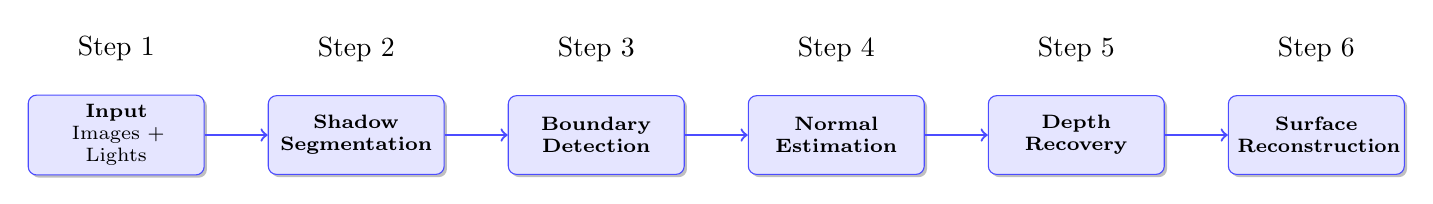
\begin{tikzpicture}[
    node distance=0.8cm,
    classicalbox/.style={rectangle, draw=blue!70, fill=blue!10, rounded corners=3pt, 
                        text width=2cm, text centered, minimum height=1cm, font=\scriptsize,
                        drop shadow={shadow xshift=1pt, shadow yshift=-1pt}},
    arrow/.style={->, thick, blue!70}
]

\node[classicalbox] (input) {\textbf{Input} \\ Images + Lights};
\node[classicalbox, right=of input] (shadow_seg) {\textbf{Shadow} \\ \textbf{Segmentation}};
\node[classicalbox, right=of shadow_seg] (boundary_det) {\textbf{Boundary} \\ \textbf{Detection}};
\node[classicalbox, right=of boundary_det] (normal_est) {\textbf{Normal} \\ \textbf{Estimation}};
\node[classicalbox, right=of normal_est] (depth_solve) {\textbf{Depth} \\ \textbf{Recovery}};
\node[classicalbox, right=of depth_solve] (surface_recon) {\textbf{Surface} \\ \textbf{Reconstruction}};

\draw[arrow] (input) -- (shadow_seg);
\draw[arrow] (shadow_seg) -- (boundary_det);
\draw[arrow] (boundary_det) -- (normal_est);
\draw[arrow] (normal_est) -- (depth_solve);
\draw[arrow] (depth_solve) -- (surface_recon);


% Timeline
\node[above=0.3cm of input] {Step 1};
\node[above=0.3cm of shadow_seg] {Step 2};
\node[above=0.3cm of boundary_det] {Step 3};
\node[above=0.3cm of normal_est] {Step 4};
\node[above=0.3cm of depth_solve] {Step 5};
\node[above=0.3cm of surface_recon] {Step 6};

\end{tikzpicture}
Figure 5: Classical method (Sequential processing pipeline)
\end{center}

\vspace{-2em}

\hypertarget{fig:neural_method}{}
\begin{center}
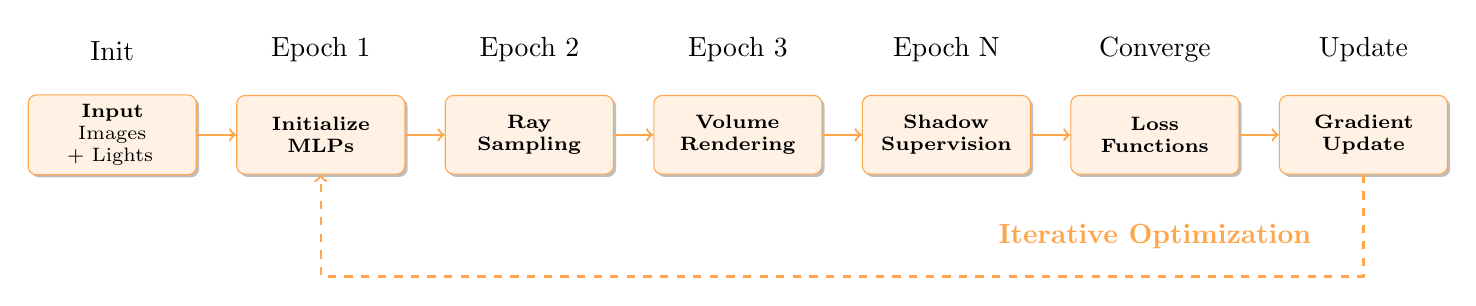
\begin{tikzpicture}[
    node distance=0.5cm,
    neuralbox/.style={rectangle, draw=orange!70, fill=orange!10, rounded corners=3pt,
                     text width=1.9cm, text centered, minimum height=1cm, font=\scriptsize,
                     drop shadow={shadow xshift=1pt, shadow yshift=-1pt}},
    arrow/.style={->, thick, orange!70},
]

\node[neuralbox] (input) {\textbf{Input} \\ Images + Lights};
\node[neuralbox, right=of input] (init_mlp) {\textbf{Initialize} \\ \textbf{MLPs}};
\node[neuralbox, right=of init_mlp] (ray_sample) {\textbf{Ray} \\ \textbf{Sampling}};
\node[neuralbox, right=of ray_sample] (volume_render) {\textbf{Volume} \\ \textbf{Rendering}};
\node[neuralbox, right=of volume_render] (shadow_super) {\textbf{Shadow} \\ \textbf{Supervision}};
\node[neuralbox, right=of shadow_super] (loss_compute) {\textbf{Loss} \\ \textbf{Functions}};
\node[neuralbox, right=of loss_compute] (gradient_update) {\textbf{Gradient} \\ \textbf{Update}};

\draw[arrow] (input) -- (init_mlp);
\draw[arrow] (init_mlp) -- (ray_sample);
\draw[arrow] (ray_sample) -- (volume_render);
\draw[arrow] (volume_render) -- (shadow_super);
\draw[arrow] (shadow_super) -- (loss_compute);
\draw[arrow] (loss_compute) -- (gradient_update);

\draw[arrow, dashed] (gradient_update) -- ++(0,-1.8) -| (init_mlp);
\node[below=of loss_compute, text=orange!70] {\textbf{Iterative Optimization}};

% Timeline
\node[above=0.3cm of input] {Init};
\node[above=0.3cm of init_mlp] {Epoch 1};
\node[above=0.3cm of ray_sample] {Epoch 2};
\node[above=0.3cm of volume_render] {Epoch 3};
\node[above=0.3cm of shadow_super] {Epoch N};
\node[above=0.3cm of loss_compute] {Converge};
\node[above=0.3cm of gradient_update] {Update};

\end{tikzpicture}
Figure 6: ShadowNeuS (End-to-end neural optimization pipeline)
\end{center}

\vspace{2em}

\begin{tabular}{p{0.4\textwidth} p{0.5\textwidth}}
\hline
\textbf{Classical Method Issues} & \textbf{Neural Solution (ShadowNeuS)} \\
\hline
\begin{itemize}[noitemsep, topsep=0pt]
    \item \textbf{Circular dependency}
    \item \textbf{Singularities}
    \item \textbf{Shadow detection}
    \item \textbf{Nonlinear equations}
\end{itemize} &
\begin{itemize}[noitemsep, topsep=0pt]
    \item \textbf{Joint learning with neural SDF}
    \item \textbf{Differentiable approximation}
    \item \textbf{Binary shadow models}
    \item \textbf{End-to-end optimization}
\end{itemize} \\
\hline
\end{tabular}

\newpage

\subsection{ShadowNeuS Pipeline} \label{sec:classical_to_neural}

In this section, we outline the complete pipeline of ShadowNeuS, from the initialization of neural SDFs to optimization using shadow supervision.

\subsubsection{Neural Signed Distance Fields (SDF)} \label{sec:neural_sdf}

\begin{definition}[Neural Signed Distance Field] \label{def:neural_sdf} ~\\
A \textbf{Neural Signed Distance Field} (Neural SDF), as introduced in \hyperlink{[PFS19]}{[PFS19]}, is a function $f(\mathbf{P}; \theta): \mathbb{R}^3 \to \mathbb{R}$ parameterized by a multi-layer perceptron (MLP) with trainable weights $\theta$. It implicitly represents a 3D scene by outputting the signed distance of any spatial point $\mathbf{P} = (p_x, p_y, p_z)^\top$ to the nearest surface:

\begin{minipage}{0.5\textwidth}
\[
\scalebox{1.05}{$
f(\mathbf{P})
\begin{cases}
< 0 & \text{if } \mathbf{P} \text{ is inside the object (blue region)}, \\
= 0 & \text{if } \mathbf{P} \text{ lies on the surface (green line)}, \\
> 0 & \text{if } \mathbf{P} \text{ is outside the object (red region)}.
\end{cases}
$}
\]
\end{minipage}
\hspace{-1em}
\begin{minipage}{0.5\textwidth}
    \begin{center}
    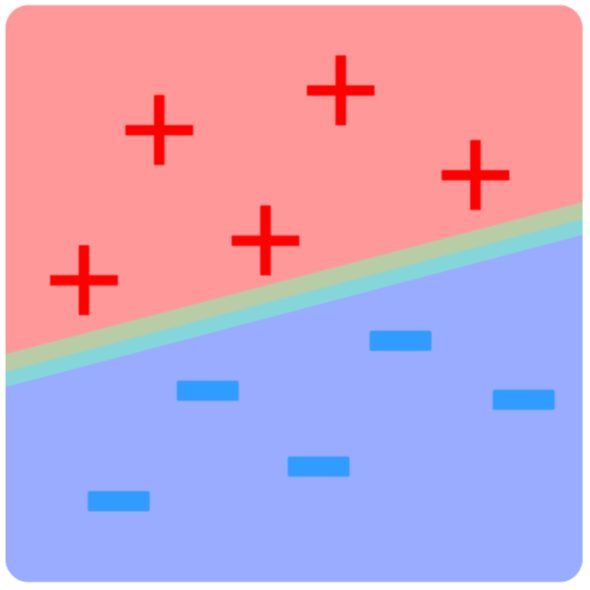
\includegraphics[height=0.17\textheight]{sdf_region.png} \\
    \textbf{Figure 7.} Signed regions of a surface \\
    \end{center}
\end{minipage}

\end{definition}

\begin{remark}[Key Properties of Neural SDF] \label{rmk:gradient_properties} ~\\
Neural SDFs encode useful geometric details for 3D reconstruction:
\begin{itemize}

    \item \textbf{Multivariable Differentiability}: The signed distance field is expressed as \( f(\mathbf{P}; \theta) \), where \(\mathbf{P}\) denotes a 3D point and \(\theta\) the neural network parameters. 
    It is differentiable with respect to both:
    \vspace{-1em}
    \[
    \begin{cases}
        \nabla_{\mathbf{P}} f(\mathbf{P}; \theta) & \text{(Use for spatial constraint or surface normal in the scene)} \\
        \nabla_{\theta} f(\mathbf{P}; \theta) & \text{(Use for gradient descent in machine learning)}
    \end{cases}
    \]

    \item \textbf{Surface Normals}: 
    On the zero level set \(f(\mathbf{P}; \theta) = 0\), the surface normal is given by the normalized spatial gradient:
    
    \begin{minipage}{0.5\textwidth}
    \begin{equation*}
    \scalebox{1.4}{$
    \hat{\mathbf{n}}(\mathbf{P}) 
    = \frac{\nabla_{\mathbf{P}} f(\mathbf{P}; \theta)}
        {\|\nabla_{\mathbf{P}} f(\mathbf{P}; \theta)\|_2}
    $}
    \end{equation*}
    \end{minipage}
    \hspace{-3em}
    \begin{minipage}{0.5\textwidth}
        \begin{center}
        \vspace{1em}
        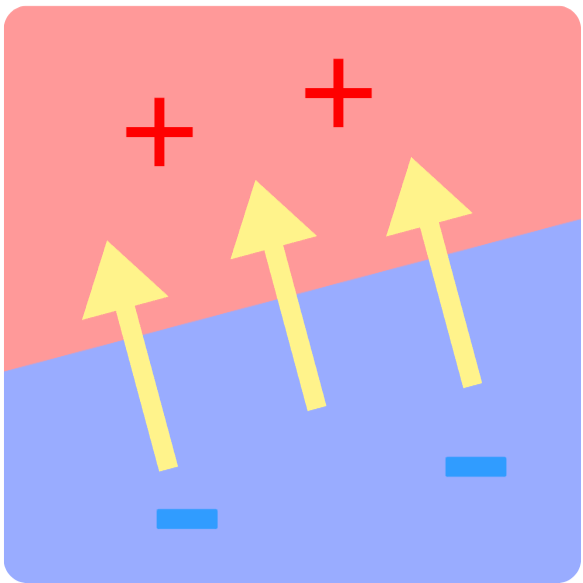
\includegraphics[height=0.17\textheight]{sdf_vec.png} \\
        \textbf{Figure 8.} The gradient of the sdf \\
        \end{center}
    \end{minipage}

    This normal is used in light–surface interactions such as shadow visibility, computed via the angle between \(\hat{\mathbf{n}}\) and the incoming light direction \(\mathbf{L} - \mathbf{P}\).

    \newpage

    \item \textbf{Eikonal Regularization (Distance Consistency)}: For $f(\mathbf{P})$ to represent a valid distance function locally, it must satisfy the \textit{Eikonal equation}:
    \begin{equation}
    \|\nabla_{\mathbf{P}} f(\mathbf{P})\|_2 = 1, \quad \forall \mathbf{P} \in \mathbb{R}^3. \label{eq:eikonal_constraint}
    \end{equation}

    \subsubsection*{Proof of Eikonal Regularization}

    Let $\mathbf{P} \in \mathbb{R}^3$ and $\mathbf{u}$ a unit vector, $\|\mathbf{u}\|_2 = 1$ and $|\sigma| \ll 1$. By first-order Taylor expansion:
    \[
    f(\mathbf{P} + \sigma \mathbf{u}) \approx f(\mathbf{P}) + \sigma \, \nabla_{\mathbf{P}} f(\mathbf{P}) \cdot \mathbf{u}.
    \]

    Let $\theta$ be the angle between $\nabla_{\mathbf{P}} f(\mathbf{P})$ and $\mathbf{u}$. Then
    \[
    \Delta f = f(\mathbf{P} + \sigma \mathbf{u}) - f(\mathbf{P}) \approx \sigma \, \nabla_{\mathbf{P}} f(\mathbf{P}) \cdot \mathbf{u} \approx \sigma \, \|\nabla_{\mathbf{P}} f(\mathbf{P})\|_2 \cos \theta.
    \]

    For $f$ to be a valid signed distance function, the change along any direction must equal the displacement:
    \[
    \Delta f = \sigma \cos \theta \quad \implies \quad \boxed{\|\nabla_{\mathbf{P}} f(\mathbf{P})\|_2 = 1}.
    \]

    \item \textbf{Geometric Stability}: Deviations from $\|\nabla_{\mathbf{P}} f(\mathbf{P})\|_2 = 1$ indicate distortion:
    \[
    \|\nabla_{\mathbf{P}} f(\mathbf{P})\|_2
    \begin{cases}
    > 1 & \text{implies local stretching (distance overestimation)}, \\
    < 1 & \text{implies local compression (distance underestimation)}.
    \end{cases}
    \]
    Enforcing the Eikonal constraint regularizes the SDF, ensuring stable and consistent geometry during optimization.
    
\end{itemize}
\end{remark}

\subsubsection{Epoch 1: Neural SDF Initialization and MLP Design} \label{sec:epoch1_neural_sdf}

The training begins by constructing a neural signed distance field (SDF), modeled by an eight-layer multi-layer perceptron (MLP) to implicitly represent 3D geometry from shadow cues. 

\begin{itemize}

    \item \textbf{Network Structure}: ShadowNeuS uses an 8-layer fully-connected MLP with ReLU activation functions, a single output head producing scalar signed distances $f(\mathbf{P}; \theta) \in \mathbb{R}$.

    \begin{remark}[Why MLP Architecture?] ~\\
    The MLP design offers several advantages:
    \begin{itemize}
        \item \textbf{Universal Approximation}: By the universal approximation theorem, MLPs can approximate any continuous function on compact subsets of $\mathbb{R}^3$.
        \item \textbf{End-to-End Differentiability}: Gradients $\nabla_{\mathbf{P}} f$, $\nabla_{\theta} f$ can be computed throughout the pipeline, enabling training directly from shadow observations.
        \item \textbf{Joint Integrative Learning}: Both surface positions ($f(\mathbf{P}) = 0$) and surface normals ($\nabla_{\mathbf{P}} f$) are jointly encoded in $f$, simplifying the learning process compared to classical pipelines which handle these separately.
        \item \textbf{Circular Dependency Resolution}: Neural SDF jointly models geometry and visibility, avoiding the iterative or circular inversion problems faced by classical shadow methods.
    \end{itemize}
    \end{remark}

    \item \textbf{Input Encoding}: To enhance the ability of the MLP to capture high-frequency geometric features, ShadowNeuS applies a sinusoidal positional encoding $\gamma(\mathbf{P})$ to the input 3D coordinates:
    \begin{equation}
    \gamma(\mathbf{P}) = \left( \sin(2^0 \pi p_x), \cos(2^0 \pi p_x), \ldots, \sin(2^{k-1} \pi p_z), \cos(2^{k-1} \pi p_z) \right).
    \end{equation}

    \begin{remark}[Why Positional Encoding?] ~\\
    Raw coordinates $\mathbf{P} = (p_x, p_y, p_z)$ do not provide sufficient high-frequency variation for MLPs, leading to overly smooth approximations (spectral bias). Positional encoding introduces Fourier feature mappings \hyperlink{[TSS20]}{[TSS20]}, allowing the network to represent both coarse and fine geometric structures revealed by shadows.
    \end{remark}

    \item \textbf{Output}: A scalar SDF value $f(\mathbf{P})$ per point.

    \item \textbf{Random Initialization}: The MLP weights $\theta$ are initialized using standard techniques such as Xavier initialization, ensuring well-scaled activations in early epochs.
\end{itemize}

% \subsubsection{Epoch 2$\to$N: Ray Sampling and Shadow Rendering} \label{sec:epoch2_ray_sampling}

% From the second epoch onward, ShadowNeuS iteratively performs \textbf{ray sampling} to locate surface points and \textbf{shadow rendering} to predict shadow values at image pixels. The procedure proceeds as follows:

% \begin{itemize}

%     \item \textbf{Camera Ray Sampling}: \\
%     For each pixel $\mathbf{p}$, a camera ray is constructed:
%     \[
%     \mathbf{r}(t) = \mathbf{C} + t \mathbf{d}, \quad \mathbf{d} = R^{-1} K^{-1} \begin{bmatrix} p_x \\ p_y \\ 1 \end{bmatrix}.
%     \]
%     The intersection point $\mathbf{P}$ is found by sphere tracing along $\mathbf{r}(t)$ to locate $t^*$ satisfying
%     \[
%     f_\theta(\mathbf{r}(t^*)) = 0, \quad \mathbf{P} = \mathbf{r}(t^*).
%     \]

%     \item \textbf{Light Ray Sampling and Visibility Estimation}: \\
%     For each $\mathbf{P}$, a light ray towards the light source $\mathbf{L}$ is defined:
%     \[
%     \mathbf{l}(s) = \mathbf{P} + s (\mathbf{L} - \mathbf{P}), \quad s \in [0, 1].
%     \]
%     The \textbf{opacity} along $\mathbf{l}(s)$ is computed at discrete points $\mathbf{l}(s_j)$ using:
%     \[
%     a_j = \max\left( 1 - \frac{ \phi(f_\theta(\mathbf{l}(s_{j+1})) ) }{ \phi(f_\theta(\mathbf{l}(s_j))) }, 0 \right)
%     \]
%     where $\phi(\cdot)$ is an active function, and $a_j \in [0,1]$ represents the \textbf{local opacity} between adjacent samples.

%     The accumulated transmittance (incoming light intensity) is then:
%     \[
%     C_{\mathrm{in}}(\mathbf{P}) = \prod_{j=1}^N (1 - a_j)
%     \]
%     This idea is inspired by Neural Radiance Fields (NeRF) C, which uses volume rendering to synthesize views from radiance fields.
% \end{itemize}

% \subsubsection{Converge: Loss Functions} \label{sec:loss_functions}

% The overall objective of the training process is to minimize a weighted sum of several loss terms that enforce both geometric and appearance-based constraints. The total loss function is defined as:
% \begin{equation}
% \mathcal{L}_{\text{total}} = w_{\text{shadow}} \cdot \mathcal{L}_{\text{shadow}} + w_{\text{eik}} \cdot \mathcal{L}_{\text{eik}} + w_{\text{app}} \cdot \mathcal{L}_{\text{appearance}} + \ldots
% \end{equation}

% \begin{itemize}
%     \item \textbf{Shadow Supervision Loss:}
%     \begin{equation}
%     \mathcal{L}_{\text{shadow}} = \sum_{\mathbf{p}} \left| C_{\mathrm{in}}(\mathbf{p}) - S(\mathbf{p}) \right|
%     \end{equation}
%     This term measures the difference between the predicted incoming light intensity $C_{\mathrm{in}}(\mathbf{p})$ and the observed shadow value $S(\mathbf{p})$ over all valid image pixels $\mathbf{p}$.

%     \item \textbf{Eikonal Loss:}
%     \begin{equation}
%     \mathcal{L}_{\text{eik}} = \frac{1}{M} \sum_{i=1}^M \left( \left\| \nabla_\mathbf{P} f(\mathbf{P}_i) \right\|_2 - 1 \right)^2
%     \end{equation}
%     This regularization ensures the predicted signed distance function (SDF) $f$ has unit gradient norm almost everywhere, encouraging smooth and well-defined surfaces.

%     \item \textbf{Appearance or Consistency Loss:}
%     \begin{equation}
%     \mathcal{L}_{\text{appearance}} = \sum_{\mathbf{p}} \left\| C_{\text{pred}}(\mathbf{p}) - C_{\text{gt}}(\mathbf{p}) \right\|_2^2
%     \end{equation}
%     This term enforces color or texture consistency by minimizing the error between predicted colors $C_{\text{pred}}$ and ground-truth colors $C_{\text{gt}}$ at pixel locations $\mathbf{p}$. Depending on the dataset, it can also include feature or texture-based losses.

%     \item \textbf{Other Loss Terms (optional):}
    
%     Additional loss terms such as normal supervision, depth alignment, or regularization losses can be added when extra supervision signals are available.
% \end{itemize}

% \subsubsection{Epoch 2$\to$N: Ray Sampling and Shadow Rendering} \label{sec:epoch2_ray_sampling}

% From the second epoch onward, ShadowNeuS performs \textbf{ray sampling} to locate surface points and \textbf{shadow rendering} to estimate shadow values at image pixels. The process has two stages:

% \begin{itemize}[noitemsep, topsep=0pt]

%     \item \textbf{Camera Ray Sampling}: \\
%     For each pixel $\mathbf{p}$, a camera ray is constructed:
%     \[
%     \mathbf{r}(t) = \mathbf{C} + t \mathbf{d}, \quad \mathbf{d} = R^{-1} K^{-1} \begin{bmatrix} p_x \\ p_y \\ 1 \end{bmatrix},
%     \]
%     where $K$ and $R$ are the intrinsic and extrinsic parameters of the camera. The intersection point $\mathbf{P}$ with the implicit surface is found by sphere tracing to locate $t^*$ such that
%     % \[
%     % f_\theta(\mathbf{r}(t^*)) \approx 0, \quad \mathbf{P} = \mathbf{r}(t^*).
%     % \]

%     \begin{minipage}{0.4\textwidth}
%     \[
%     \scalebox{1}{$
%     f_\theta(\mathbf{r}(t^*)) \approx 0, \quad \mathbf{P} = \mathbf{r}(t^*).
%     $}
%     \]
%     \end{minipage}
%     \hspace{-1em}
%     \begin{minipage}{0.5\textwidth}
%         \begin{center}
%         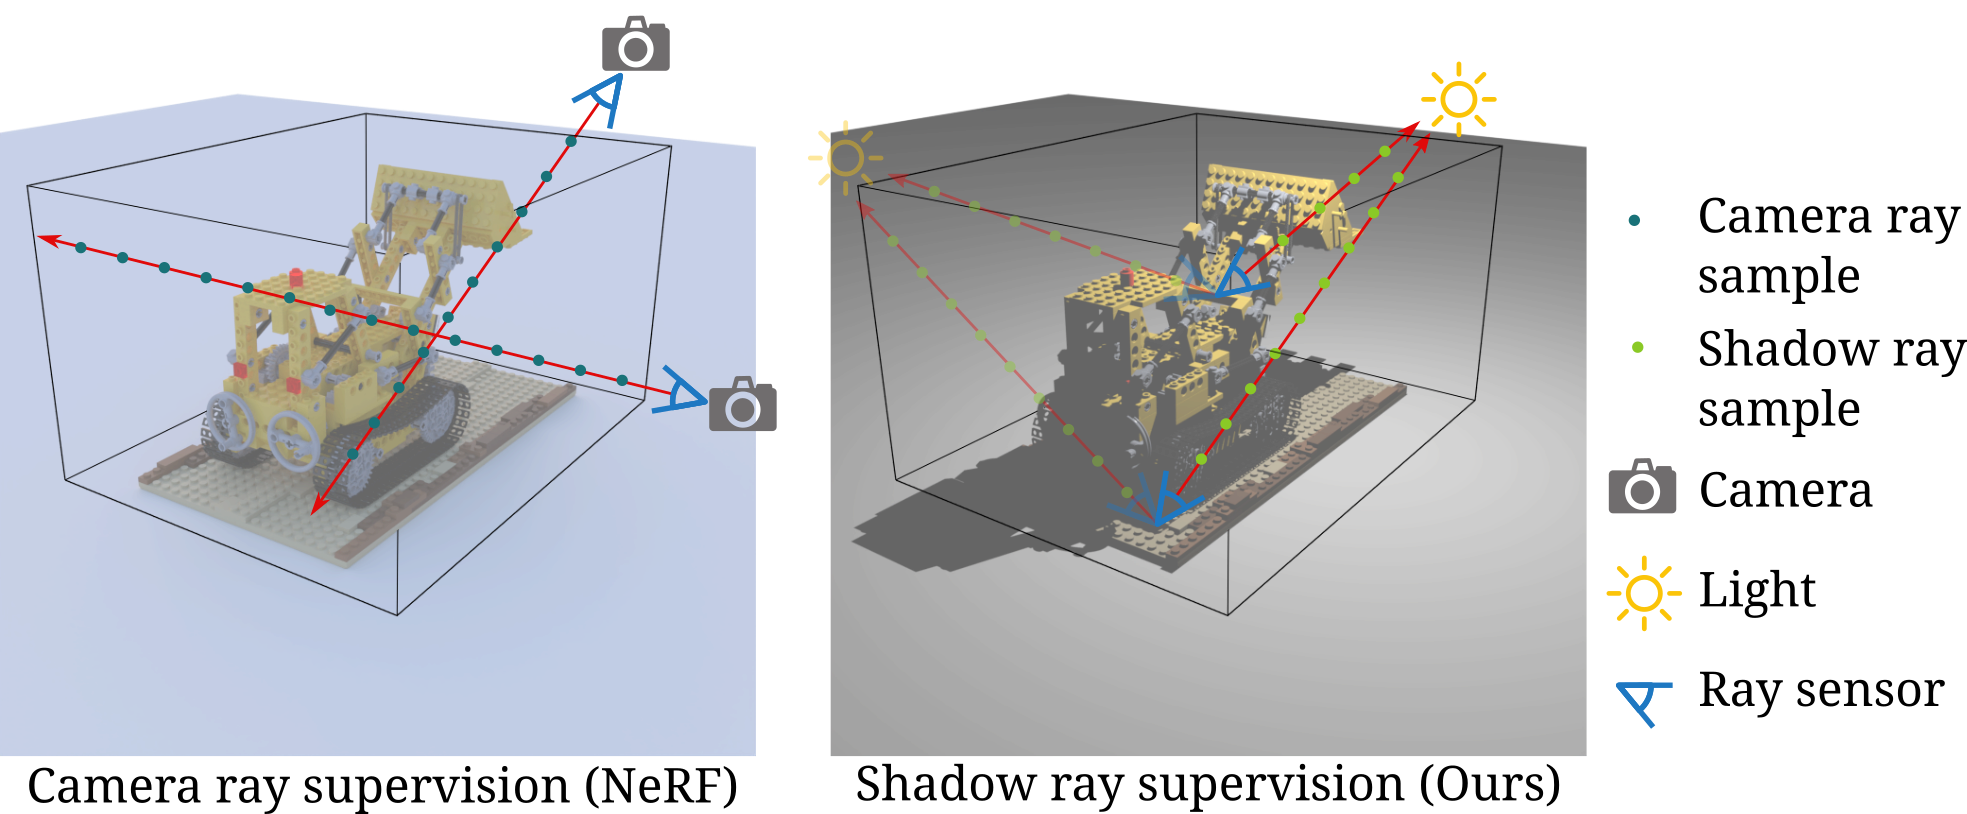
\includegraphics[height=0.16\textheight]{shadowneus_rays.png} \\
%         \textbf{Figure 9.} Comparision between \\ Camera ray and Shadow ray \hyperlink{[LWX23]}{[LWX23]} \\
%         \end{center}
%     \end{minipage}

% \newpage

%     \item \textbf{Light Ray Sampling and Visibility Estimation}: \\
%     For each surface point $\mathbf{P}$, a light ray toward the light source $\mathbf{L}$ is defined:
%     \[
%     \mathbf{l}(s) = \mathbf{P} + s (\mathbf{L} - \mathbf{P}), \quad s \in [0, 1].
%     \]
%     Along this ray, discrete samples $\mathbf{l}(s_j)$ are taken to evaluate visibility. A local opacity between samples is computed as
%     \[
%     a_j = \max\left( 1 - \frac{ \phi(f_\theta(\mathbf{l}(s_{j+1})) ) }{ \phi(f_\theta(\mathbf{l}(s_j))) }, 0 \right),
%     \]
%     where $\phi(\cdot)$ is a smooth mapping from signed distance to positive density (e.g., softplus). Each $a_j \in [0,1]$ represents the \textbf{local opacity} between adjacent points.

%     The accumulated transmittance, representing the incoming light at $\mathbf{P}$, is then
%     \[
%     C_{\mathrm{in}}(\mathbf{P}) = \prod_{j=1}^N (1 - a_j).
%     \]
%     This multiplicative accumulation is analogous to volume rendering used in NeRF \hyperlink{[MST20]}{[MST20]}, where densities are integrated along rays to estimate visibility in a differentiable way.
% \end{itemize}


\subsubsection{Epoch 2$\to$N: Ray Sampling and Shadow Rendering} \label{sec:epoch2_ray_sampling}

From the second epoch onward, ShadowNeuS performs \textbf{ray sampling} to locate surface points and \textbf{shadow rendering} to estimate shadow values at image pixels. The process has two stages:

\begin{itemize}[noitemsep, topsep=0pt]
    \item \textbf{Camera Ray Sampling}: \\
    For each pixel $\mathbf{p}$, a camera ray is constructed:
    \[
    \mathbf{r}(t) = \mathbf{C} + t \mathbf{d}, \quad \mathbf{d} = R^{-1} K^{-1} \begin{bmatrix} p_x \\ p_y \\ 1 \end{bmatrix},
    \]
    where $K$ and $R$ are the intrinsic and extrinsic parameters of the camera. The intersection point $\mathbf{P}$ with the implicit surface is found by sphere tracing to locate $t^*$ such that
    \[
    f_\theta(\mathbf{r}(t^*)) \approx 0, \quad \mathbf{P} = \mathbf{r}(t^*).
    \]

    \item \textbf{Shadow Ray Sampling and Visibility Estimation}: \\ 
    For each $\mathbf{P}$, a light ray towards the light source $\mathbf{L}$ is defined:
    \[
    \mathbf{l}(s) = \mathbf{P} + s (\mathbf{L} - \mathbf{P}), \quad s \in [0, 1].
    \]
    The \textbf{opacity} along $\mathbf{l}(s)$ is computed at discrete points $\mathbf{l}(s_j)$ using:
    \[
    a_j = \max\left( 1 - \frac{ \phi(f_\theta(\mathbf{l}(s_{j+1})) ) }{ \phi(f_\theta(\mathbf{l}(s_j))) }, 0 \right)
    \]
    where $\phi(\cdot)$ is an active function, and $a_j \in [0,1]$ represents the \textbf{local opacity} between adjacent samples.

    The accumulated transmittance (incoming light intensity) is then:
    \[
    C_{\mathrm{in}}(\mathbf{P}) = \prod_{j=1}^N (1 - a_j)
    \]
    This multiplicative accumulation is analogous to volume rendering used in NeRF \hyperlink{[MST20]}{[MST20]}, where densities are integrated along rays to estimate visibility in a differentiable way.
    \begin{center}
        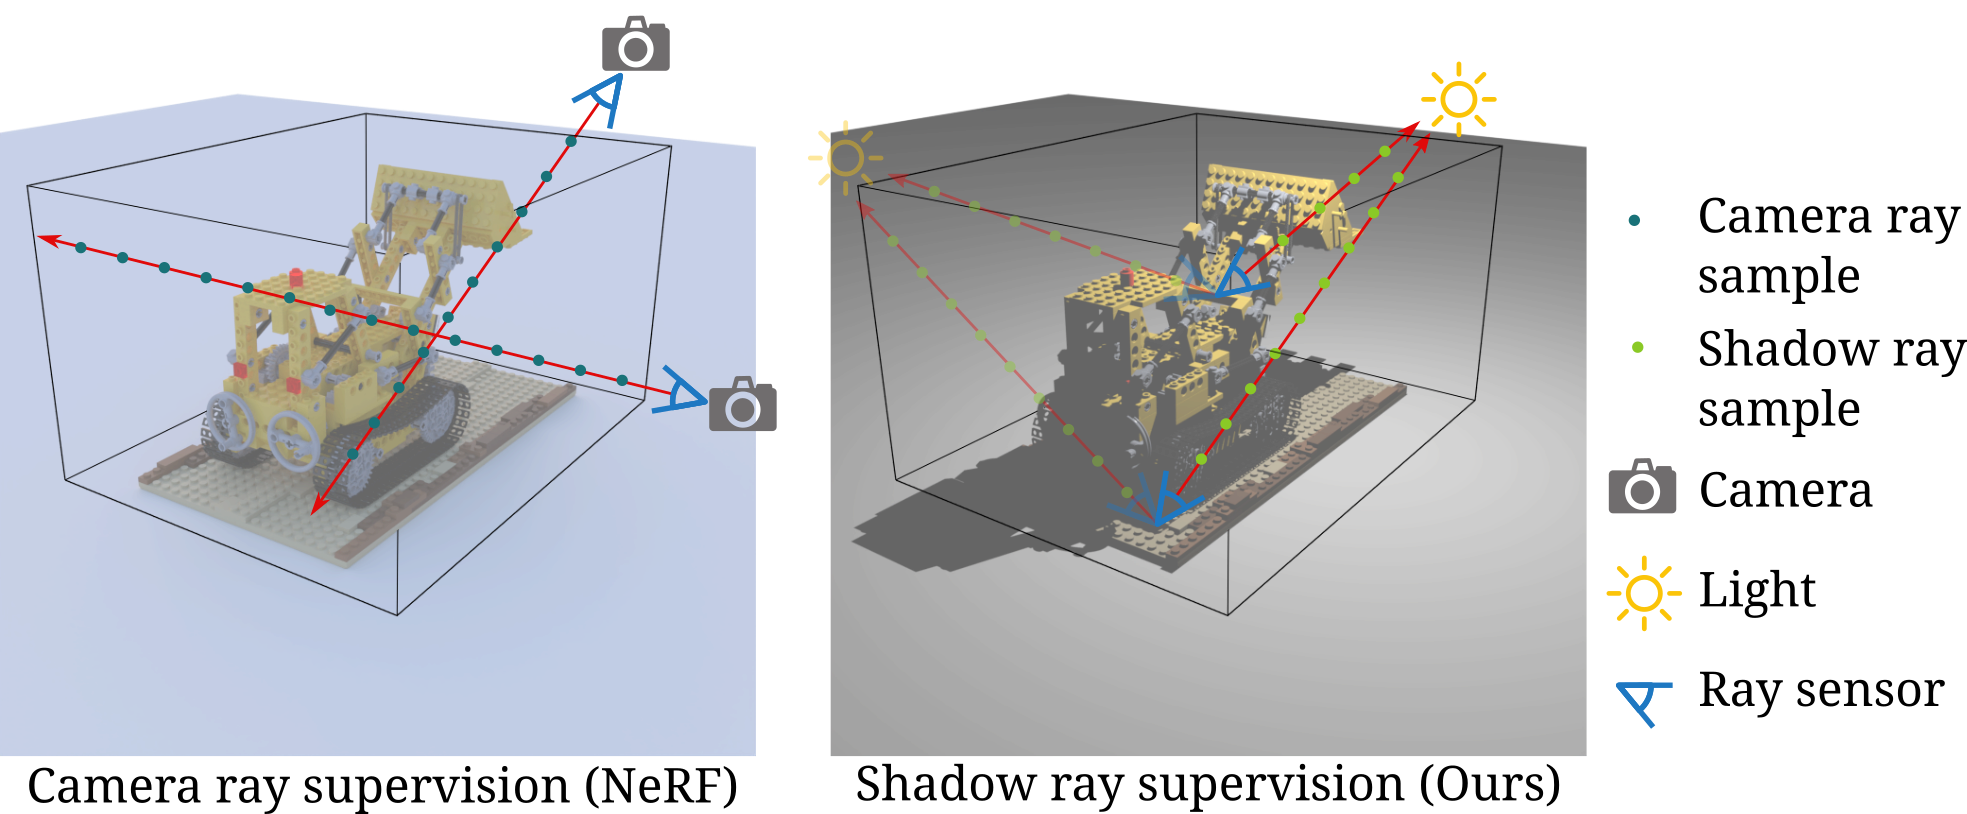
\includegraphics[width=0.7\textwidth]{shadowneus_rays.png} \\
        \textbf{Figure 9.} Comparision between Camera ray and Shadow ray \hyperlink{[LWX23]}{[LWX23]}
    \end{center}

\end{itemize}

\subsubsection{Convergence: Loss Functions} \label{sec:loss_functions}

Training minimizes a weighted sum of several loss terms that enforce geometric regularity and appearance consistency:
\begin{equation*}
\mathcal{L}_{\text{total}} = w_{\text{shadow}} \cdot \mathcal{L}_{\text{shadow}} + w_{\text{eik}} \cdot \mathcal{L}_{\text{eik}} + w_{\text{app}} \cdot \mathcal{L}_{\text{appearance}} + \ldots
\end{equation*}

\begin{itemize}
    \item \textbf{Shadow Supervision Loss:}
    \begin{equation*}
    \mathcal{L}_{\text{shadow}} = \sum_{\mathbf{p}} \left| C_{\mathrm{in}}(\mathbf{p}) - S(\mathbf{p}) \right|
    \end{equation*}
    compares predicted light transmittance $C_{\mathrm{in}}(\mathbf{p})$ with observed shadow labels $S(\mathbf{p})$.

    \item \textbf{Eikonal Loss:}
    \begin{equation*}
    \mathcal{L}_{\text{eik}} = \frac{1}{M} \sum_{i=1}^M \left( \left\| \nabla_\mathbf{P} f_\theta(\mathbf{P}_i) \right\|_2 - 1 \right)^2
    \end{equation*}
    encourages $f_\theta$ to approximate a signed distance function by enforcing unit-norm gradients almost everywhere, leading to stable and smooth surfaces.

    \item \textbf{Appearance or Consistency Loss:}
    \begin{equation*}
    \mathcal{L}_{\text{appearance}} = \sum_{\mathbf{p}} \left\| C_{\text{pred}}(\mathbf{p}) - C_{\text{gt}}(\mathbf{p}) \right\|_2^2
    \end{equation*}
    enforces consistency between predicted and ground-truth colors (or features) at each pixel. Depending on the dataset, this may include texture or feature-based terms.

    \item \textbf{Other Loss Terms (optional):} \\
    When additional supervision is available, terms such as normal alignment, depth consistency, or regularization losses can be added.
\end{itemize}

\subsubsection{Gradient Descent and Adam Optimizer} \label{sec:adam_optimizer}

To minimize the total loss $\mathcal{L}_{\text{total}}(\theta)$, neural networks typically rely on gradient-based optimization methods. Below, we summarize both the basic gradient descent method and the more advanced Adam optimizer used in our implementation. Details of Adam optimizer are refered to paper \hyperlink{[KB14]}{[KB14]}.

\begin{itemize}

    \item \textbf{Gradient Descent}: The simplest optimization method updates the parameters $\theta$ along the direction of steepest descent, defined by the negative gradient of the loss:
    \[
    \theta_{t+1} = \theta_t - \alpha \, \nabla_\theta \mathcal{L}_{\text{total}}(\theta_t),
    \]
    where $\theta_t$ denotes the parameters at iteration $t$, $\alpha > 0$ is the \textbf{learning rate}, and $\nabla_\theta \mathcal{L}_{\text{total}}$ is the gradient of the total loss with respect to $\theta$.

    \begin{remark}[Limitations of Simple Gradient Descent]
    Despite its simplicity, basic gradient descent exhibits several limitations:
    \begin{itemize}
        \item \textbf{Learning Rate Sensitivity}: A fixed $\alpha$ may result in slow convergence (if too small) or divergence (if too large).
        \item \textbf{Oscillation}: In regions with steep or curved loss landscapes, updates can oscillate and hinder convergence.
        \item \textbf{Uniform Step Size}: All parameters are updated using the same learning rate, without accounting for variations in gradient magnitude.
    \end{itemize}
    \end{remark}

    \item \textbf{Adam Optimizer}: Adaptive Moment Estimation (Adam) addresses these issues by combining:
    \begin{itemize}
        \item \textbf{Momentum (First Moment Estimate)}: Adam maintains an exponentially decaying average of past gradients:
        \[
        m_t = \beta_1 m_{t-1} + (1 - \beta_1) g_t, \quad g_t = \nabla_\theta \mathcal{L}_{\text{total}}(\theta_t),
        \]
        where $0 < \beta_1 < 1$ controls the momentum decay. This term reduces oscillations and stabilizes updates.

        \item \textbf{Adaptive Scaling (Second Moment Estimate)}: Adam also tracks the exponentially decaying average of squared gradients:
        \[
        v_t = \beta_2 v_{t-1} + (1 - \beta_2) g_t^2,
        \]
        where $0 < \beta_2 < 1$ governs the decay rate for squared gradients. This adjusts learning rates per parameter based on historical gradient magnitudes.

        \item \textbf{Bias Correction}: To correct for initialization bias (since $m_0, v_0 = 0$), Adam computes bias-corrected estimates:
        \[
        \hat{m}_t = \frac{m_t}{1 - \beta_1^t}, \quad \hat{v}_t = \frac{v_t}{1 - \beta_2^t}.
        \]
    \end{itemize}

    \item \textbf{Adam Update Rule}: The final parameter update rule is given by:
    \[
    \theta_{t+1} = \theta_t - \alpha \cdot \frac{\hat{m}_t}{\sqrt{\hat{v}_t} + \epsilon},
    \]
    where:
    \begin{itemize}
        \item $\alpha$ is the learning rate (e.g., $\alpha = 10^{-3}$),
        \item $\beta_1$ is the first moment decay rate (typically $\beta_1 = 0.9$),
        \item $\beta_2$ is the second moment decay rate (typically $\beta_2 = 0.999$),
        \item $\epsilon$ is a small constant (e.g., $\epsilon = 10^{-8}$) to ensure numerical stability and prevent division by zero.
    \end{itemize}

\end{itemize}







\section{Experimental Demonstration}
% ...

\section{Discussion and Analysis}
% ...

\section{Conclusion}
% ...


\section*{References}
\spaceskip=0.3em plus 0.1em minus 0.1em
\begin{tabular}{p{0.15\textwidth}p{0.85\textwidth}}
{[LWX23]}               & Jingwang Ling, Zhibo Wang, Feng Xu. \textit{ShadowNeuS: Neural SDF Reconstruction by Shadow Ray Supervision}. arXiv: \href{https://arxiv.org/abs/2211.14086}{2211.14086}, 2023. \hypertarget{[LWX23]}{}  \\
{[VK23]}                & Venkatkumar. \textit{3D Reconstruction Basic Terminology (Traditional Computer Vision Approach)}. Medium: \href{https://medium.com/@VK_Venkatkumar/3d-reconstruction-basic-terminology-traditional-computer-vision-e148496f389}{URL}, 2023. \hypertarget{[VK23]}{} \\
{[\textbf{Figure 1.}]}  & Sjoerd van Riel. \textit{Exploring the use of 3D GIS as an analytical tool in archaeological excavation practice}. ResearchGate: \href{https://www.researchgate.net/figure/Structure-from-Motion-SfM-photogrammetric-principle-Source-Theia-sfmorg-2016_fig3_303824023}{URL}, 2016. \hypertarget{[Fig 1]}{} \\
{[\textbf{Figure 2.}]}  & Catree. \href{https://stackoverflow.com/questions/38494485/camera-coordinate-to-pixel-coordinate-opencv}{Camera coordinate to pixel coordinate - OpenCV}, 2016. \hypertarget{[Fig 2]}{} \\
{[\textbf{Figure 3.}]}  & Lemanoosh. \href{https://lemanoosh.com/online-course-blender-material-rendering/}{Blender material rendering}, n.d. \hypertarget{[Fig 3]}{}  \\
{[\textbf{Figure 4.}]}  & Michael Abramov. \href{https://keymakr.com/blog/semantic-segmentation-vs-object-detection-understanding-the-differences/}{Semantic Segmentation vs Object Detection: Understanding the Differences}, 2024. \hypertarget{[Fig 4]}{}  \\
{[\textbf{Figure 5.}]}  & Sandip Neogi. \href{https://www.vecteezy.com/vector-art/42399612-shadow-of-object}{shadow of object Pro Vector}, n.d. \hypertarget{[Fig 5]}{}  \\
{[\textbf{SHFP01}]}     & S. Savarese, H. Rushmeier, F. Bernardini, P. Perona. \textit{Shadow Carving} IEEE:\href{https://ieeexplore.ieee.org/document/937517}{10.1109/ICCV.2001.937517}, 2001. \hypertarget{[SHFP01]}{}  \\
{[\textbf{M51}]}        & Gaspard Monge. \textit{An Elementary Treatise on Descriptive Geometry, with a Theory of Shadows and of Perspective Extracted from the French of G. Monge by J. F. Heather} Google book id: \href{https://archive.org/details/bub_gb_8KZ0SKUCVXQC/page/n17/mode/2up}{8KZ0SKUCVXQC}, 1851. \hypertarget{[M51]}{}  \\
{[\textbf{PFS19}]}      & Jeong Joon Park, Peter Florence, Julian Straub, Richard Newcombe, Steven Lovegrove. \textit{DeepSDF: Learning Continuous Signed Distance Functions for Shape Representation}. arXiv: \href{https://arxiv.org/abs/1901.05103}{1901.05103}, 2019. \hypertarget{[PFS19]}{}\\
{[\textbf{TSS20}]}      & Matthew Tancik, Pratul P. Srinivasan, Ben Mildenhall, Sara Fridovich-Keil, Nithin Raghavan, Utkarsh Singhal, Ravi Ramamoorthi, Jonathan T. Barron, Ren Ng. \textit{Fourier Features Let Networks Learn High Frequency Functions in Low Dimensional Domains}. arXiv: \href{https://arxiv.org/abs/2006.10739}{2006.10739}, 2020. \hypertarget{[TSS20]}{}\\
{[\textbf{MST20}]}      & Ben Mildenhall, Pratul P. Srinivasan, Matthew Tancik, Jonathan T. Barron, Ravi Ramamoorthi, Ren Ng. \textit{NeRF: Representing Scenes as Neural Radiance Fields for View Synthesis}. arXiv: \href{https://arxiv.org/abs/2003.08934}{2003.08934}, 2020. \hypertarget{[MST20]}{}\\
{[\textbf{KB14}]}       & Diederik P. Kingma, Jimmy Ba. \textit{Adam: A Method for Stochastic Optimization}. arXiv: \href{https://arxiv.org/abs/1412.6980}{1412.6980}, 2014. \hypertarget{[KB14]}{}\\
\end{tabular}


\end{document}